\CQUsection{实验与结果分析}

\CQUsubsection{实验设计概述}
本文实验以动脉瘤分割和破裂风险预测两个方面为研究对象，从体素级病灶识别能力、病例级风险判别能力两个方面来对所提出的方法进行系统的评价。分割实验用CTA三维体数据作为输入，考查模型输出的概率图和人工标注的掩膜之间的一致性；风险预测实验用临床信息、影像表型信息、分割衍生特征作为输入，考查模型对动脉瘤破裂状态的区分能力。虽然两项任务在输入形式、输出目标和评价粒度上存在不同之处，但是它们共同服务于颅内动脉瘤智能分析这一总体目标，即在影像结构识别的基础上进一步实现风险评估。

本文在实验组织上严格遵守了训练集、验证集、测试集三者互不干扰的基本原则。训练集用来做模型参数的学习，验证集用来做超参数调节、阈值确定和模型选择，测试集只用来做最终性能的评价，以最小化信息泄漏造成的偏差。本文主要从分割任务的角度出发，对模型在训练后期的收敛稳定性、概率判别能力以及病灶检出能力进行了研究。对于风险预测任务，本文主要对比了深度交叉注意力模型和传统的机器学习模型在多项评价指标上的表现，并且对不同模型的判别特点和适用场景进行了分析。

\CQUsubsection{实验环境及基本设置}
实验是在通用Linux计算环境下完成的，深度学习模型使用主流张量计算框架进行训练和推理，医学影像读取、空间重采样、数值计算和统计分析都依靠成熟的科学计算工具来完成。为了保证实验过程的可重复性，所有的实验都是在统一的数据划分、统一的评价口径、一致的训练和验证流程下进行记录的。本文在结果分析中主要对模型表现和方法学意义进行探讨，而不涉及具体的工程实现细节。

输入是三维CTA体数据。训练阶段使用局部补丁学习方法来解决显存限制问题，提高小目标病灶在训练过程中可见性；验证阶段使用滑窗方式进行整例推理，保证输出结果有空间完整性。风险预测任务输入是病例级表格特征，数值变量做标准化处理，类别变量做离散嵌入表示，模型输出为病例级破裂概率。考虑到风险预测任务中正负样本分布一般存在不平衡情况，本文在训练阶段使用类别加权策略，在验证集上搜索最优判别阈值，提升模型对于少数类样本的识别能力。

保证比较的公平性，所有的对比模型都采用相同的划分方式，测试集不参与训练、调参和阈值选择。分割实验中模型选择主要根据验证集的重叠指标和阳性检出能力来决定；风险预测实验中，阈值选择只根据验证集输出概率完成，之后将该阈值固定在测试集上报告性能。该设计可以减小由于测试集反馈所造成的乐观偏差，使实验结果更真实地反映出模型对于未见样本的泛化表现。

从统计学习的角度来说，实验设计的主要问题就是把模型选择过程和最终的性能评价过程分开。训练集、验证集、测试集分别记为 $\mathcal{D}_{tr}$、$\mathcal{D}_{val}$、$\mathcal{D}_{te}$，模型参数由训练集确定：
\begin{equation}
\hat{\theta}=\arg\min_{\theta}\frac{1}{|\mathcal{D}_{tr}|}\sum_{(x_i,y_i)\in\mathcal{D}_{tr}}\mathcal{L}(x_i,y_i;\theta),
\label{eq:train-obj}
\end{equation}
其中$\mathcal{L}$ 是损失函数，比如交叉熵损失或本文中使用的组合损失。
超参数和阈值由验证集决定：
\begin{equation}
\hat{\gamma}=\arg\max_{\gamma\in\Gamma}S_{val}(\hat{\theta},\gamma),
\label{eq:val-select}
\end{equation}
其中$S_{val}$ 是验证集的评价函数，比如 Dice 系数、F1 值、AUC 等。$\ gamma$ 是模型选择过程中所选择的超参数。

最终性能只在测试集上计算：
\begin{equation}
S_{test}=S(\mathcal{D}_{te};\hat{\theta},\hat{\gamma}).
\label{eq:test-score}
\end{equation}
γ可以是分类阈值、模型结构选择或者验证集选择等。上述形式化的描述指出，测试集不能被任何模型选择过程所影响，否则会造成性能估计偏乐观。

医学数据一般存在病例间异质性、标注不确定性和类别分布不均等，因此不能用一个指标来全面地表现模型的行为。本文在分割任务中同时考虑区域重叠、阳性检出、概率排序，在风险预测任务中同时考虑总体判别、阳性识别、阈值敏感性，从而减少由于使用单一评价标准而产生的解释偏差。

\CQUsubsection{评价指标}
\CQUsubsubsection{分割任务评价指标}
分割任务评价要从概率判别能力、区域重叠程度和阳性体素检出能力三方面来考虑。设真实前景集合为 $Y$，预测前景集合为 $\hat{Y}$，Dice 系数定义为
\begin{equation}
\mathrm{Dice}=\frac{2|Y\cap \hat{Y}|}{|Y|+|\hat{Y}|}.
\label{eq:eval-dice}
\end{equation}
Dice 系数越大，说明预测区域和真实区域的重叠程度越大。由于动脉瘤一般体积小，边界的微小偏差就会造成 Dice 明显的波动，所以该指标对于分割质量比较敏感。

从体素级二分类的角度出发，真阳性、假阳性、真阴性和假阴性分别记作TP、FP、TN和FN。召回率定义为
\begin{equation}
\mathrm{Recall}=\frac{\mathrm{TP}}{\mathrm{TP}+\mathrm{FN}},
\label{eq:eval-recall}
\end{equation}
用来衡量真实前景体素被正确识别出来的比例。对于医学筛查场景来说，召回率具有重要的意义，因为漏检病灶会直接导致后续的临床判断失误。精确率定义为
\begin{equation}
\mathrm{Precision}=\frac{\mathrm{TP}}{\mathrm{TP}+\mathrm{FP}},
\label{eq:eval-precision}
\end{equation}
用来衡量预测为前景的体素中真实属于前景的比例。另外，Precision 和 Recall 的调和平均可以表示为
\begin{equation}
F_1=\frac{2\times \mathrm{Precision}\times \mathrm{Recall}}{\mathrm{Precision}+\mathrm{Recall}}.
\label{eq:eval-f1}
\end{equation}
AUC 用阈值无关的方式描述模型对前景和背景体素的整体排序能力，可以用来刻画概率输出的可分性。如果用真阳性率TPR(τ)和假阳性率FPR(τ)分别表示阈值τ下敏感度和误报率，那么ROC-AUC就可以形式化地表示为
\begin{equation}
\mathrm{AUC}=\int_{0}^{1}\mathrm{TPR}\left(\mathrm{FPR}^{-1}(u)\right)du,
\label{eq:eval-auc}
\end{equation}
此式用于解释在所有的可能的阈值下，综合评价模型把前景体素排序在背景体素之前的能力。

考虑到小目标分割中边界少量偏差会造成较大指标波动，本文主要以 Dice、Recall、F1 与 AUC 为核心指标，并结合可视化结果讨论边界误差。

\CQUsubsubsection{风险预测评价指标}
风险预测属于病例级不平衡二分类问题，因此只用Accuracy来评价模型是不够全面的。Accuracy定义为
\begin{equation}
\mathrm{Accuracy}=\frac{\mathrm{TP}+\mathrm{TN}}{\mathrm{TP}+\mathrm{TN}+\mathrm{FP}+\mathrm{FN}},
\label{eq:accuracy}
\end{equation}
反映整体分类正确率，但是在正负样本比例失衡时会忽略模型对少数类样本的识别情况。因此本文同时给出Precision、Recall、F1和AUC等指标来全面反映模型在风险识别任务上的表现。

对于风险预测模型输出的概率 $\hat{p}_i$，其二分类结果由阈值 $\tau$ 决定：
\begin{equation}
\hat{y}_i=
\begin{cases}
1, & \hat{p}_i\geq \tau,\\
0, & \hat{p}_i<\tau.
\end{cases}
\label{eq:risk-threshold}
\end{equation}
本文在验证集上搜索较优阈值，并将其固定用于测试集评估。该策略可以利用数据分布以及任务目标自动调整决策边界，从而降低默认阈值对于实验结果的影响。以F1值作为选择准则时，可以写成
\begin{equation}
\tau^{\ast}=\arg\max_{\tau\in[0,1]}\frac{2\mathrm{Precision}(\tau)\mathrm{Recall}(\tau)}{\mathrm{Precision}(\tau)+\mathrm{Recall}(\tau)}.
\label{eq:best-threshold}
\end{equation}

除此之外，医学风险预测还要考虑概率输出的可解释性和校准性。理想情况下，当模型对一组病例给出接近 $p$ 的风险概率时，该组病例中实际阳性比例也应该接近 $p$。将样本按照预测概率分成 $K$ 个区间 $B_k$，则期望校准误差可以表示为
\begin{equation}
\mathrm{ECE}=\sum_{k=1}^{K}\frac{|B_k|}{N}\left|\operatorname{acc}(B_k)-\operatorname{conf}(B_k)\right|,
\label{eq:ece}
\end{equation}
其中 $\operatorname{acc}(B_k)$ 是第 $k$ 个区间内的真实阳性比例，$\operatorname{conf}(B_k)$ 是平均预测概率。虽然本文主要对分类判别指标进行报告，但是校准分析对于后续的临床使用有着非常重要的意义，因为风险概率不仅会改变二分类决策，还会改变临床复核、随访优先级的安排。

为了方便说明各类评价指标在本文中所起的作用，对本章主要指标以及它们的分析侧重点进行了归纳。

\begin{table}[htbp]
\centering
\caption{主要评价指标及其分析侧重点}
\label{tab:metric_summary}
\small
\begin{tabular}{lll}
\toprule
任务类型 & 指标 & 主要反映内容 \\
\midrule
分割任务 & Dice & 预测区域与真实区域的重叠程度 \\
分割任务 & Recall & 病灶前景体素的检出能力 \\
分割任务 & Precision & 前景预测结果的可靠性 \\
分割任务 & AUC & 前景与背景体素的整体可分性 \\
风险预测任务 & Accuracy & 整体分类正确率 \\
风险预测任务 & Precision & 高风险预测结果的准确性 \\
风险预测任务 & Recall & 破裂病例的识别能力 \\
风险预测任务 & F1 & Precision 与 Recall 的综合平衡 \\
风险预测任务 & AUC & 破裂与未破裂病例的排序能力 \\
\bottomrule
\end{tabular}
\normalsize
\end{table}

\CQUsubsection{动脉瘤分割实验}
\CQUsubsubsection{实验目的与训练过程}

分割实验的主要目的是检验三维 Attention U-Net 及其改进结构对颅内动脉瘤的定位能力以及轮廓恢复能力。训练时，模型用局部补丁样本学习病灶及其邻域的空间结构，在验证和测试阶段对整例 CTA 体数据进行滑窗推理。由于动脉瘤在空间上非常稀疏，实验不但重视病灶前景的召回率，还重视在复杂的血管背景下的误检控制。从训练过程来看，模型在后期的验证指标逐渐趋于稳定，说明网络已经基本完成从低层纹理到高层病灶语义的表征学习。本文主要统计了该阶段的验证结果，来观察收敛末期的性能表现。在此期间，AUC 和 Recall 均处于相对稳定的区间，说明模型对于前景和背景的概率排序能力较强，而且病灶检出性能没有出现明显的波动。从训练过程上来说，模型在后期的验证指标逐渐趋于稳定，说明网络已经基本完成了从低层纹理到高层病灶语义的表征学习。本文主要对这一阶段的验证结果进行统计，以观察收敛末期的性能表现。在此期间，AUC 和 Recall 均保持在相对稳定的区间，说明模型对于前景和背景的概率排序能力较强，而且病灶检出性能没有出现明显的波动。除此之外，训练过程还体现出小目标分割中“概率排序”和“空间成形”的区别。前者强调模型是否可以给真实的病灶体素赋予比背景更高的概率，后者则关注在阈值化之后是否可以形成连续、解剖合理的三维区域。如果模型 AUC 高但 Dice 低，一般认为其概率排序能力已经较好，但是阈值化后的分割结果会出现边界收缩、离散假阳性或者局部漏检的情况。因此，在训练后期，除了关注损失函数和 AUC 外，还需要结合固定阈值下的 Dice、Recall 以及可视化结果，综合判断模型是否具备稳定的空间分割能力。


\CQUsubsubsection{分割结果和阈值分析}
以较好的验证轮次为例，在阈值0.5的情况下模型得到AUC为0.97、Recall为0.56的结果，说明模型在当前的验证数据上已经具有较好的体素级区分能力。以最终检查点为报告对象，在相同的阈值下AUC为0.96、Recall为0.55，和较好的轮次表现接近，说明训练后期模型并没有出现明显的退化，整体的泛化性能并没有出现明显的下降。

需要指出的是，较高的AUC并不能说明分割结果在空间上已经达到了完全理想的状态。AUC主要用来评价不同的阈值下模型对于正负体素整体排序的质量，但是最终二值掩膜的空间一致性还会受到阈值选择、病灶体积、边界清晰度和重建方式等影响。对于小目标病灶来说，虽然模型在概率排序上表现良好，但是不恰当的阈值仍然会造成边界收缩、局部断裂或者离散误检区域。因此对分割模型进行评价的时候应该把Dice、Recall以及典型病例的可视化结果结合起来分析，而不是仅仅依靠一个指标来判断。

从阈值扫描结果可知，分割阈值 $\tau_s$ 越大，模型预测越保守，误检体素数目会减少，但是Recall会同步下降；反之，当阈值减小时，模型会倾向于保留低置信度的疑似前景，Recall会增加，但是误检风险也会增加。其决策形式可以表示为
\begin{equation}
\hat{M}_{i,j,k}(\tau_s)=\mathbb{I}\left(P_{i,j,k}\geq \tau_s\right).
\label{eq:threshold-decision}
\end{equation}

其中，$\hat{M}_{i,j,k}(\tau_s)$ 表示模型对第 $i$ 行第 $j$ 列第 $k$ 个体素的预测结果，$P_{i,j,k}$ 表示模型对第 $i$ 行第 $j$ 列第 $k$ 个体素的概率。当 $\tau_s$ 增大时，满足条件的前景集合会越来越小，漏检概率也随之增大。对于医学辅助分析场景来说，保持较高的病灶检出能力很重要，但是同时也要控制误检区域的大小，保证后续结构定量分析以及临床展示的可解释性。

\CQUsubsubsection{可视化分析与误差来源}
从典型的病例可视化结果可知，模型对于大部分病灶区域能够较好地覆盖动脉瘤主体，在局部边界上形成比较连续的响应。对于形态比较规则、对比度比较高的病灶来说，预测掩膜和人工标注的一致性较高；但是当病灶体积小、边缘对比度低、与载瘤血管过渡模糊或者邻近高密度结构干扰明显的时候，模型就会出现局部漏检、边界偏移或者少量误检。

这类误差具有一定的普遍性。一方面，小病灶在多次下采样过程中容易造成空间信息的丢失，即使使用跳跃连接进行细节的补充，也还不能完全恢复极细小结构边界；另一方面，CTA中血管增强区域和动脉瘤前景在灰度分布上存在相似性，模型需要依靠空间上下文和拓扑关系而不是仅仅依靠强度差异来做出判断。因此，如果后续要提高分割效果，可以就更具针对性的前景采样、边界敏感损失设计、多尺度监督以及稳健的后处理策略等角度进行优化。

从误差分解的角度来说，分割误差可以分为阈值误差、边界误差和结构误差三类。阈值误差主要是由于概率输出和二值决策不一致造成的；边界误差主要是预测轮廓相对于真实轮廓的局部偏移；结构误差就是病灶区域断裂、漏检或者与邻近血管粘连。设预测概率为 $P$，真实标签为 $Y$，阈值化结果为 $\hat{M}(\tau_s)$，则不同阈值下的分割质量可以表示为
\begin{equation}
S(\tau_s)=\mathcal{M}\left(\hat{M}(\tau_s),Y\right),
\label{eq:threshold-quality}
\end{equation}
其中 $\mathcal{M}(\cdot)$ 表示任一分割评价指标。若 $S(\tau_s)$ 在较宽的阈值区间内保持稳定，则说明模型概率图具有较好的校准性、空间鲁棒性；若指标随着阈值剧烈波动，则说明模型输出中存在大量的低置信度或者边界不确定区域。

对于动脉瘤分割而言，误差分析还要考虑空间位置和解剖背景。病灶与载瘤血管交界处一般是容易发生边界偏移的地方，因为二者在增强影像上灰度分布接近，而且真实标注也受观察者经验的影响。邻近骨性结构、高密度伪影或者血管分叉区域容易产生假阳性响应。以上现象说明，模型性能的提高不能只依靠更复杂的网络结构，还需要从数据表示、监督信号以及评价方式上共同约束。

\CQUsubsubsection{分割模型消融分析}
为了分析模型性能提升的来源，本文从结构设计角度对分割模型进行了消融讨论。可以把基础三维 Attention U-Net、引入 ASPP 的增强模型、进一步加入三维坐标注意力的模型作为逐步增强的结构序列。基础模型主要是依靠编码器—解码器结构和注意力门控来完成病灶的恢复；ASPP模块用多尺度空洞卷积扩大感受野，有利于增强模型对不同尺度病灶及其邻域上下文的刻画能力；三维坐标注意力又加入了方向感知的位置建模，对边界模糊、形态不规则或者空间走向复杂的病灶有潜在的优势。

从现有的实验结果可以看出，增强模型比基础模型具有更好的综合分割性能。在相同的训练轮次下，ASPP-CA-UNet的Recall为0.67，AUC为0.96，比基础模型Dice系数提高约20%，F1值提高约40%。两类模型对于大多数背景体素来说都具有较高的一致性，说明增强模型性能的提高并不是由于对背景的过度拟合造成的，而更可能是由于对病灶区域表征能力的提高所导致的。为了方便比较，表~\ref{tab:seg_ablation}对分割消融结果进行了汇总。

\begin{table}[htbp]
\centering
\caption{分割模型消融结果比较}
\label{tab:seg_ablation}
\small
\begin{tabular}{lcccc}
\toprule
模型 & Recall & AUC & Dice（相对变化） & F1（相对变化） \\
\midrule
基础三维 Attention U-Net & 0.56 & 0.97 & 基准水平 & 基准水平 \\
Attention U-Net + ASPP + CA & 0.67 & 0.96 & +20\% & +40\% \\
\bottomrule
\end{tabular}
\normalsize
\end{table}

由于动脉瘤分割属于一种高度不平衡的体素级任务，背景体素占的比例远大于病灶体素，所以整体像素一致性会受到很多真阴性体素的主导，其解释力比较小。相比之下，Dice、Recall、F1等更能反映病灶区域识别能力的指标，可以更真实地反映模型在本任务上的性能差异。因此本文在消融分析时更重视结构对病灶区域识别质量的改善，而不是单纯地关注整体一致性指标。

ASPP和坐标注意力的作用机制以及增益来源不同。ASPP用不同的空洞率并行分支来扩大感受野，主要提高模型对于不同尺度病灶以及其周围血管背景上下文的理解能力；坐标注意力则是通过对空间方向信息的建模来加强位置感知，更适合处理走向复杂或者边界模糊的血管结构。只引入多尺度特征而缺少位置约束，模型容易对背景血管做出过大的响应；反之，如果只加入位置注意力而缺少多尺度上下文，那么对于形态变化大的病灶的适应性就会较差。因此这两类模块在理论上是互补的，联合使用可以更好地解决小目标分割中背景抑制和结构保持的问题。


若用 $S_0$ 表示基础模型性能，用 $S_A$ 表示加入 ASPP 后的性能，用 $S_{A+C}$ 表示同时加入 ASPP 与坐标注意力后的性能，则各模块的边际贡献可形式化表示为
\begin{align}
\Delta_{A} &= S_A-S_0,\\
\Delta_{C\mid A} &= S_{A+C}-S_A.
\end{align}
$\Delta_A$ 体现的是多尺度上下文增强直接带来的贡献，$\Delta_{C\mid A}$ 表示的是在已经有了多尺度表示的基础上，方向注意力带来的增量效果。如果两个模块都是正的，说明两个模块对于目标指标有累积的增益；如果单独增益较弱但是联合增益明显，则可能存在互补作用。本文实验结果表明，增强结构在Dice和F1上相对提高的幅度更大，说明其主要改善的是前景区域重叠的质量和阳性预测可靠性，而不仅仅是概率排序能力。

\CQUsubsection{破裂风险预测实验}
\CQUsubsubsection{实验目的与模型设置}
破裂风险预测实验用以评价多源表格特征对于病例级破裂状态的判别能力，同时比较交叉注意力模型和传统机器学习模型在中小规模医学数据条件下的表现。所有模型都使用相同的训练集、验证集、测试集划分来评估，验证集上完成阈值选择，保证各个模型之间有共同的比较基础。

本文所包含的比较模型有交叉注意力深度表格模型、随机森林、逻辑回归、支持向量机、$k$近邻以及融合模型。逻辑回归可以看作是线性可解释的基线，随机森林是集成树模型，支持向量机和 $k$近邻分别是基于核映射和局部相似性的传统分类方法，而交叉注意力模型是利用字段交互学习高阶依赖关系的深度方法。融合模型把树模型和注意力模型的输出结合起来，用来检验不同模型范式之间的互补性。

\CQUsubsubsection{对比实验结果}
风险预测模型测试集结果见表~\ref{tab:risk_result}。表中 Threshold 表示由验证集确定并固定用于测试集评估的分类阈值。

\begin{table}[htbp]
\centering
\caption{风险预测模型测试集对比结果}
\label{tab:risk_result}
\small
\setlength{\tabcolsep}{4pt}
\resizebox{\textwidth}{!}{%
\begin{tabular}{lcccccc}
\toprule
模型 & Accuracy & Precision & Recall & F1 & AUC & Threshold \\
\midrule
Forest-Attention Ensemble & 0.7944 & 0.6931 & 0.7778 & \textbf{0.7330} & \textbf{0.8568} & 0.350 \\
Risk Cross-Attention & 0.7852 & 0.6832 & 0.7667 & 0.7266 & 0.8546 & 0.325 \\
Random Forest & 0.7419 & 0.6182 & 0.7556 & 0.6800 & 0.8284 & 0.400 \\
Logistic Regression & 0.6895 & 0.5512 & 0.7778 & 0.6452 & 0.7342 & 0.450 \\
KNN & 0.5766 & 0.4576 & \textbf{0.9000} & 0.6067 & 0.6966 & 0.200 \\
SVM-RBF & 0.5565 & 0.4451 & \textbf{0.9000} & 0.5956 & 0.6732 & 0.300 \\
\bottomrule
\end{tabular}%
}
\normalsize
\end{table}

根据表~\ref{tab:risk_result}可知，Forest-Attention Ensemble在测试集上获得最高的F1值0.7330和AUC值0.8568，说明传统树模型和深度注意力模型在当前任务中具有一定的互补优势。Risk Cross-Attention模型得到F1值为0.7266、AUC值为0.8546，其性能与最优融合模型相差不大，明显优于逻辑回归、支持向量机、k近邻等传统单模型基线。基于字段级交互的深度建模方式可以很好地捕捉到临床变量和影像表型变量之间非线性关系。

从随机森林在Accuracy、F1和AUC等指标上都比很多传统基线好可以看出集成树模型对于中小规模表格数据的稳定性以及适应性。相比之下，KNN和SVM-RBF模型虽然Recall达到0.9000，有较强的阳性病例检出倾向，但是它们的Precision分别是0.4576和0.4451，F1以及AUC也都处在较低水平。这说明这两类模型更倾向于把样本判定为高风险类别，虽然可以提高召回能力，但是也明显增加了误报率，整体结果并没有超过随机森林或者随机森林-注意力融合模型。逻辑回归虽然具有很强的可解释性，但是它的AUC只有0.7342，线性决策边界很难很好地刻画出当前多源特征中复杂的非线性关系。

从模型假设的角度来说，不同的方法之间的区别可以归结为判别函数空间的不同。逻辑回归对应线性形式
\begin{equation}
\log\frac{\hat{p}}{1-\hat{p}}=\beta_0+\sum_{j}\beta_jx_j,
\end{equation}

其中$\hat{p}$ 表示预测的概率，$\beta_j$ 表示变量 $x_j$ 的权重，$\beta_0$ 表示常数项。它的优点是参数意义明确，但是不能自动表达高阶非线性交互。随机森林用多个决策树的集成形成分段非线性判别函数，可以较好的处理变量之间的条件分裂关系。交叉注意力模型用字段token之间注意力权重的学习来得到全局交互，其判别函数可以抽象为
\begin{equation}
\hat{p}=\sigma\left(F_{\omega}(e_1,e_2,\ldots,e_{m+q})\right),
\label{eq:cross-attn-risk}
\end{equation}
其中 $F_{\omega}(\cdot)$ 表示由多层注意力和非线性映射构成的可学习函数， $e_i$ 表示第 $i$ 个字段的表示向量，$m$ 表示临床特征数量，$q$ 表示影像特征数量。该类模型具有更强的表达能力，但是对样本规模、正则化和数据噪声更敏感。因此，实验结果中深度模型与集成树模型表现接近，符合中小规模医学表格数据的一般规律。

\CQUsubsubsection{阈值选择与不平衡分类讨论}

风险预测实验中各个模型的最优阈值都小于或者接近于0.5，说明默认的判别阈值不能很好地适应医学风险识别任务的实际需要。对于输出概率 $\hat{p}$ 而言，降低阈值会使更多的病例被判定为高风险，从而提高 Recall，但是也会降低 Precision；提高阈值会产生相反的效果。因此，阈值选择本质上是在漏诊风险和误报代价之间做出取舍。

从临床辅助分析的角度来说，破裂风险预测一般会关注高风险病例的检出能力，因此Recall比其他的属性更有参考价值，但是当Precision较低的时候，就会出现过多的低风险病例被误判为高风险的情况，进而加重后续检查、复核和干预的负担。F1值是通过综合考虑Precision和Recall来给动脉瘤破裂风险预测的二分类任务提供一个更平衡的评价方式。AUC是用全阈值范围来反映模型对于阳性、阴性病例排序的能力，可以用来比较模型之间的总体判别能力。

进一步地，阈值选择可以被看作是代价敏感的决策问题。假阴性代价为 $C_{FN}$，假阳性代价为 $C_{FP}$，当给定预测概率 $\hat{p}$ 时，病例判定为阳性的期望代价为 $C_{FP}(1-\hat{p})$，判定为阴性的期望代价为 $C_{FN}\hat{p}$。当 $C_{FP}(1-\hat{p}) < C_{FN}\hat{p}$ 时，选择阳性判定更合理。由此可得理论阈值
\begin{equation}
\tau_c=\frac{C_{FP}}{C_{FP}+C_{FN}}.
\end{equation}
当漏诊代价大于误报代价时，$C_{FN}>C_{FP}$，对应的阈值 $\tau_c$ 小于 0.5，这与实验中多个模型的最优阈值小于默认阈值的现象相符。由此可知，阈值不是单纯的参数，它反映了具体应用场景中漏诊和误报之间的取舍。

\CQUsubsubsection{风险模型结果讨论}

从各个指标来看，基于交叉注意力的深度表格模型在本次任务中具有较强的竞争力，但是并没有全面超过所有的传统方法。主要是由于交叉注意力机制可以显式地捕捉到异构字段之间复杂的依赖关系，在处理多源医学表格数据的时候有较好的表达能力；另一方面，在样本规模较小的情况下，传统的集成学习模型一般会比其他的模型有较好的稳健性，并且过拟合的风险也较低。

因此，深度模型和传统模型之间不是简单的替代关系，而是根据不同的数据条件和评价目标而各有千秋。融合模型在本实验中取得最优综合性能，该结果又进一步证明了上述的判断。由此可知，使用树模型的分裂规则以及使用注意力机制的表示学习，实际上捕捉到了不同的判别模式，二者结合起来可以一定程度上缓解单一模型的偏差，从而提高整体分类效果。也给后面探索更系统的模型融合策略提供支持，有利于进一步提高风险预测的稳定性以及泛化能力。

从误差类型上看，假阴性、假阳性在风险预测任务中有着不同的临床意义。假阴性是指高风险病例被低估，容易造成复查、干预等时机的延误；假阳性是指低风险病例被高估，容易造成不必要的随访负担和临床资源的浪费。因此，在该任务中不能只追求 Accuracy，而应该根据具体的临床场景来权衡 Recall、Precision 和 F1 等指标的相对重要性。本实验中，部分模型通过降低阈值获得较高的 Recall，但是 Precision 明显下降，说明它对于阳性类别的概率输出比较敏感，但是缺乏足够的可靠性。相比之下，交叉注意力模型和融合模型在 Precision 与 Recall 之间取得更加均衡的表现，综合评价指标也更高。

同时，当前结果也表明要小心地去理解深度表格模型的优势。当样本量小、变量噪声大或者阳性比例小的时候，复杂的模型就很容易学到和训练分布有关但是泛化能力差的模式。因此，较高的测试集指标还需要配合置信区间、重复划分或者外部验证来进一步验证。本文实验结果表明交叉注意力模型有较好的风险判别能力，但是其临床稳定性还需要在更大的规模数据和更严格的验证条件下进一步研究。

\CQUsubsection{结果综合讨论}

根据综合分割、风险预测实验结果可知，本文方法在目前数据集上已经形成了从影像结构识别到病例风险估计的完整分析流程。分割模型在体素级AUC和Recall上表现稳定，说明它可以把病灶和复杂的血管背景很好地区分开来；风险预测模型在F1和AUC上接近最优融合模型，说明交叉注意力机制在多源表格特征建模中具有较好的适用性。

从方法构成上讲，分割任务用注意力门控、ASPP、三维坐标注意力分别实现了背景抑制、多尺度上下文聚合、方向位置建模，三者一起提高了模型对于复杂血管结构的表达能力。在风险预测任务中，字段级嵌入和交叉注意力机制把传统的特征拼接转变成可以学习的交互表示，使模型在病例层面可以捕捉临床变量、影像表型、形态特征之间的潜在依赖关系。

同时也会出现一些值得注意的问题。医学影像数据规模小、标注成本高、单次数据划分结果容易受到样本分布的影响等；风险预测任务中的类别不平衡问题会严重影响到阈值的选择和指标的解读；深度表格模型在中小样本医学任务中并不总是稳定优于传统集成模型，合理的正则化、特征选择、概率校准以及外部验证仍然需要。

\CQUsubsection{系统展示}
为了保证整个方法流程的完整性，本文把分割推理、特征提取和风险预测组织成一个端到端的演示系统。该系统可以从输入CTA影像开始，依次完成病灶概率图生成、二值掩膜输出、形态特征提取以及破裂风险概率估计，最后以可视化的方式呈现关键结果。

\begin{figure}[htbp]
    \centering
    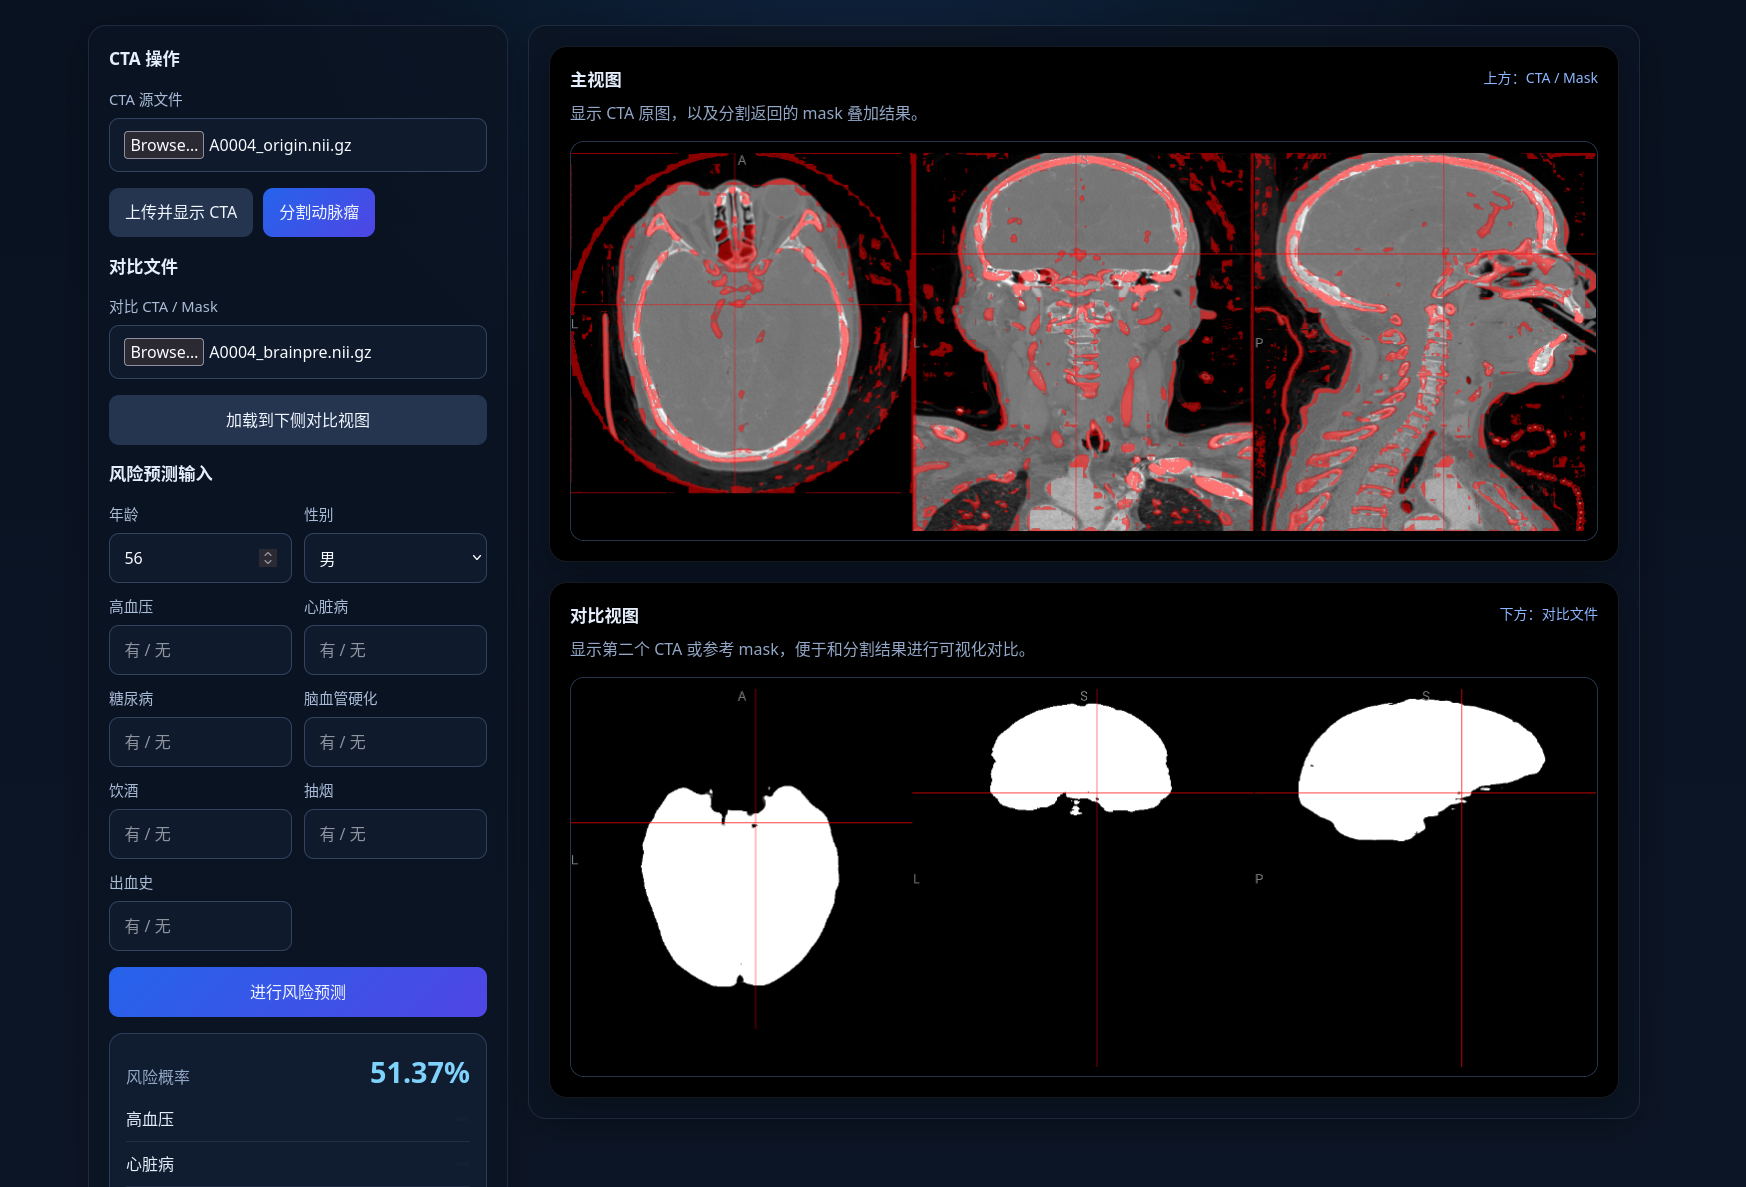
\includegraphics[width=0.8\linewidth]{figure/display.png}
    \caption{系统展示界面}
    \label{fig:display_picture}
\end{figure}

如图~\ref{fig:display_picture}所示，系统界面主要包含以下几个功能模块：影像上传模块用于接收用户上传的CTA体数据，并展示在用户界面中，位于界面右上角部分；分割推理模块调用训练好的三维Attention U-Net模型对输入影像进行动脉瘤区域识别，在此过程中会流式分割CTA的三维体数据，之后进行单独patch预测并拼装后返回给用户界面展示；风险预测模块将形态特征与临床信息结合，通过交叉注意力模型输出病例级破裂风险概率。


\CQUsubsection{本章小结}
本章从实验设计、评价指标、分割实验、风险预测对比、消融分析以及结果讨论等几个方面对本文的方法进行了比较系统的实验性评价。结果表明，分割模型在当前的验证数据上具有较好的体素级判别能力以及病灶检出能力；风险预测模型可以有效地利用多源表格特征，在测试集上取得接近最优融合模型的综合表现。本文方法在病灶识别和风险评估两个方面基本达到了预期目标，但是稳健性、泛化性等的检测和提升还需要通过大规模、多中心的多轮重复实验来进一步验证和完善。